
% The \phantomsection command is needed to create a link to a place in the document that is not a
% figure, equation, table, section, subsection, chapter, etc.
% https://tex.stackexchange.com/questions/44088/when-do-i-need-to-invoke-phantomsection
\phantomsection

% Multiple-language document - babel - selectlanguage vs begin/end{otherlanguage}
% https://tex.stackexchange.com/questions/36526/multiple-language-document-babel-selectlanguage-vs-begin-endotherlanguage


\chapter{Resultados}
\label{cap_resultados}
%\renewcommand{\topfraction}{.75}
%\renewcommand{\floatpagefraction}{.95}
%\renewcommand{\textfraction}{.75}

Utilizando a metodologia descrita no \autoref{cap_metodologia}, foram executadas uma série de ensaios de aquisição, transmissão e processamento de dados utilizando uma \textit{Merging Unit} comercial com o intuito de validar os métodos propostos no \autoref{cap_algoritmos}. 

\section{Equipamentos Utilizados}

O equipamento utilizado como fonte de tensão e corrente foi a fonte de referência \textit{Fluke 6100A} \cite{fluke6100a}. Este dispositivo é amplamente utilizado para a calibração de equipamentos de medição presentes em sistemas de energia elétrica, sendo assim a fonte ideal para estes ensaios.

A \textit{Merging Unit} utilizada nos ensaios possui três tipos de placas de aquisição analógica: duas de proteção, com 1A e 5A de correntes de entrada nominais, e uma de medição, com 1A de corrente nominal. Nos ensaios descritos neste capítulo, foi utilizada uma placa de aquisição deste terceiro modelo, por conta de ser a placa que possui especificações de precisão mais rígidas. Todos os três modelos possuem 115V de tensão nominal, 50/60Hz de frequência nominal e oito canais de aquisição, sendo quatro de corrente e quatro de tensão. Na tabela \ref{tab:specsMEA} estão descritas as especificações de precisão de corrente desta placa e na tabela \ref{tab:specsMEV} as especificações de tensão.

\begin{table}[H]
\IBGEtab{
  \caption[Especificações de Corrente de entrada para a placa de aquisição utilizada.]{Especificações de Corrente de entrada para a placa de aquisição utilizada.}
  \label{tab:specsMEA}
}{%
  \begin{tabular}{ccc}
  \toprule
   \textbf{Faixa de amplitude (A)} & \textbf{Erro} & \textbf{Erro de Fase} \\
  \midrule
   0.05In ... 0.2In       & < 0.6 \% rd     & < $\pm$ $0.3^{\circ}$  \\
  \midrule
   0.2In ... 0.8In        & < $\pm$ 0.2 \%  rd & < $\pm$ $0.15^{\circ}$  \\
  \midrule
  0.8In ... 4In           & < $\pm$ 0.1 \% rd & < $\pm$ $0.1^{\circ}$ \\
  \midrule
  4In ... 40In           & < $\pm$ 0.4 \%  rd & < $\pm$ $0.2^{\circ}$ \\
  \bottomrule
\end{tabular}
}{
  \fonte{Produzido pelo autor.}
  \nota{rd representa o valor lido (em A).}
 % regressão linear. -- \showfont}%
  %\nota[Anotações]{Uma anotação adicional, que pode ser seguida de várias
  %outras. -- \showfont}%
  }
\end{table}


\begin{table}[H]
\IBGEtab{%
  \caption[Especificações de Tensão de entrada para a placa de aquisição utilizada.]{Especificações de Tensão de entrada para a placa de aquisição utilizada.}%
  \label{tab:specsMEV}
}{%
  \begin{tabular}{ccc}
  \toprule
   \textbf{Faixa de amplitude (V)} & \textbf{Erro} & \textbf{Erro de Fase} \\
  \midrule
   0.08Vn ... 2Vn       & < 0.1\% rd     & < $\pm$ $0.1^{\circ}$  \\
  \bottomrule
\end{tabular}%
}{%
  \fonte{Produzido pelo autor.}%
  \nota{rd representa o valor lido (em V).}
  %\nota{Esta é uma nota, que diz que os dados são baseados na
 % regressão linear. -- \showfont}%
  %\nota[Anotações]{Uma anotação adicional, que pode ser seguida de várias
  %outras. -- \showfont}%
  }
\end{table}

Por serem de medição, os sinais aplicados nas entradas desta placa são amostrados 256 vezes por ciclo, trazendo 15360 amostras por segundo.

A \textit{Merging Unit} escolhida para estes experimentos possui apenas dois parâmetros de calibração: ganho e \textit{offset}. Isso vale dizer que, na prática, é possível apenas calibrar estas placas de aquisição com linearizações de primeira ordem.

\section{Sinais Aplicados}

Com o intuito de cobrir o máximo das faixas de aquisição do equipamento, os ensaios foram efetuados aplicando os seguintes sinais, cada qual com a duração de 2s:

\begin{itemize}
    \item 9.2V e 0.05A (8\% da tensão nominal e 5\% da corrente nominal);
    \item 57V e 0.2A (49\% da tensão nominal e 20\% da corrente nominal);
    \item 92V e 1A (80\% da tensão nominal e 100\% da corrente nominal);
    \item 115V e 1.2A (100\% da tensão nominal e 120\% da corrente nominal);
    \item 138V e 3A (120\% da tensão nominal e 300\% da corrente nominal);
    \item 161V e 4A (140\% da tensão nominal e 400\% da corrente nominal).
\end{itemize}

Estes ensaios foram executados para as frequências de 50Hz e 60Hz. Apesar das especificações da \textit{Merging Unit} utilizada não trazer informações sobre os erros relacionados à frequência do sinal amostrado, esta variedade de frequências foi utilizada pois na norma que define os requisitos para as \textit{Merging Units} \cite{IEC61869-13}, há uma série de especificações e restrições em termos de frequência do sinal aplicado.

\section{Erros antes das calibrações}

A fim de expor os erros antes das calibrações de maneira objetiva, mas que contenham a quantidade de detalhes necessária para a análise antes e após a aplicação dos métodos de calibração, foram escolhidos um canal de tensão e um de corrente. De forma arbitrária, foram escolhidos o canal VC de tensão e o canal IA de corrente para uma análise mais aprofundada. Esta escolha foi tomada pois todos os canais são iguais por projeto, o que tira a necessidade de uma análise particular para cada um dos quatro canais de corrente ou para cada um dos quatro canais de tensão da placa.

As tabelas \ref{tab:tabelaerros60A} e \ref{tab:tabelaerros60V} mostram os erros máximos, mínimos e médios entre os valores aplicados pela fonte de referência em 60Hz nos canais de corrente IA e de tensão VC e o sinal obtido a partir do fluxo de dados (registro no formato COMTRADE) gerado pela \textit{Merging Unit} antes de qualquer calibração. 

\begin{table}[H]
\IBGEtab{%
  \caption[Sinais de corrente em 60Hz aplicados do canal de corrente IA e os erros observados no COMTRADE gerado]{Sinais de corrente em 60Hz aplicados do canal de corrente IA e os erros observados no COMTRADE gerado.}%
  \label{tab:tabelaerros60A}
}{%
\begin{tabular}{cccccccc}
  %\small -> diminuir fonte
  \toprule
   & & & \textbf{Canal IA} &  & &  \\
  \midrule
  \textbf{Val. Apl. (mA)} & \textbf{Err. Máx.} & \textbf{Valor Máx.} & \textbf{\%} & \textbf{Valor Mín.} & \textbf{\%} & \textbf{Valor Méd.} & \textbf{\%}  \\
  \midrule
  50 & 0.6 \% & 49.6972 & -0.6054 & 50.0724 &  0.1449 & 49.9492 & -0.1015 \\
  \midrule
  200  & 0.2 \% &198.4886 &	-0.7557 &	198.8362 &	-0.5819	 & 198.6554 &-0.6723   \\
  \midrule
  1000 & 0.1 \% & 992.5441 &	-0.7456 & 996.3666 & -0.3633 & 994.4909 & -0.5509 \\
  \midrule
  1200 & 0.1 \% & 1191.3389 & -0.7218 & 1195.8324 & -0.3473 &	1193.9886 &	-0.501 \\
  \midrule
  3000 & 0.1 \% & 2977.7406 &	-0.7427	& 2986.4467 & -0.4518 & 2980.7856 & -0.6405 \\
  \midrule
  4000 & 0.1 \% & 3970.6934 &	-0.7327	& 3984.9192 & -0.377 & 3976.2538 & -0.5937 \\
  \bottomrule
\end{tabular}%
}{%
  \fonte{Produzido pelo autor.}%
 % \nota{rd representa o valor lido (em V).}
  %\nota{Esta é uma nota, que diz que os dados são baseados na
 % regressão linear. -- \showfont}%
  %\nota[Anotações]{Uma anotação adicional, que pode ser seguida de várias
  %outras. -- \showfont}%
  }
\end{table}

\begin{table}[H]
\IBGEtab{%
  \caption[Sinais de tensão em 60Hz aplicados do canal de tensão VC e os erros observados no COMTRADE gerado]{Sinais de tensão em 60Hz aplicados do canal de tensão VC e os erros observados no COMTRADE gerado.}%
  \label{tab:tabelaerros60V}
} & \textbf{Valor Mín.} & \textbf{\%} & \textbf{Valor Méd.} & \textbf{\%}  \\
  \midrule
  9.2 & 0.1 \% & 9.0365 & -1.7776 & 9.1038 & -1.046 & 9.0721 & -1.3905 \\
  \midrule
  57 & 0.1 \% & 56.5918 & -0.7161 & 56.6886 & -0.5464 & 56.6271	& -0.6542   \\
  \midrule
  92 & 0.1 \% & 90.5461 & -1.5804 & 90.8937 & -1.2025 & 90.7219	& -1.3892 \\
  \midrule
  115 & 0.1 \% & 113.212 & -1.5548 & 113.6297 & -1.1915 & 113.462 & -1.3374 \\
  \midrule
  138 & 0.1 \% & 135.8283 & -1.5737 & 136.2215 & -1.2887 & 135.9616 & -1.4771 \\
  \midrule
  161 & 0.1 \% & 158.4674 & -1.573 & 159.0317 & -1.2225 & 158.6857 & -1.4374 \\
  \bottomrule
\end{tabular}%
}{%
  \fonte{Produzido pelo autor.}%
 % \nota{rd representa o valor lido (em V).}
  %\nota{Esta é uma nota, que diz que os dados são baseados na
 % regressão linear. -- \showfont}%
  %\nota[Anotações]{Uma anotação adicional, que pode ser seguida de várias
  %outras. -- \showfont}%
  }
\end{table}

As tabelas \ref{tab:tabelaerros50A} e \ref{tab:tabelaerros50V} mostram os erros máximos, mínimos e médios entre os valores aplicados pela fonte de referência agora em 50Hz nos mesmos canais IA e VC, antes das calibrações.

\begin{table}[H]
\IBGEtab{%
  \caption[Sinais de corrente em 50Hz aplicados do canal de corrente IA e os erros observados no COMTRADE gerado]{Sinais de corrente em 50Hz aplicados do canal de corrente IA e os erros observados no COMTRADE gerado.}%
  \label{tab:tabelaerros50A}
} & \textbf{Valor Mín.} & \textbf{\%} & \textbf{Valor Méd.} & \textbf{\%}  \\
  \midrule
  50 & 0.6 \% & 45.6652 & -8.6697 & 53.3063 & 6.6126 & 46.606 & -6.7879 \\
  \midrule
  200 & 0.2 \% & 181.3421 & -9.329 & 183.8014 & -8.0993 & 183.6756 & -8.1622\\
  \midrule
  1000 & 0.1 \% & 906.9636 & -9.3036 & 918.6465 & -8.1353 & 915.047 & -8.4953\\
  \midrule
  1200 & 0.1 \% & 1088.7455 & -9.2712 & 1100.1593 & -8.3201 & 1095.6554 & -8.6954\\
  \midrule
  3000 & 0.1 \% & 2721.4705 & -9.2843 & 2756.0831 & -8.1306 & 2740.8389 & -8.6387\\
  \midrule
  4000 & 0.1 \% & 3629.1494 & -9.2713 & 3678.0604 & -8.0485 & 3654.2462 & -8.6438 \\
  \bottomrule
\end{tabular}%
}{%
  \fonte{Produzido pelo autor.}%
 % \nota{rd representa o valor lido (em V).}
  %\nota{Esta é uma nota, que diz que os dados são baseados na
 % regressão linear. -- \showfont}%
  %\nota[Anotações]{Uma anotação adicional, que pode ser seguida de várias
  %outras. -- \showfont}%
  }
\end{table}

\begin{table}[H]
\IBGEtab{%
  \caption[Sinais de tensão em 50Hz aplicados do canal de tensão VC e os erros observados no COMTRADE gerado]{Sinais de tensão em 50Hz aplicados do canal de tensão VC e os erros observados no COMTRADE gerado.}%
  \label{tab:tabelaerros50V}
} & \textbf{Valor Mín.} & \textbf{\%} & \textbf{Valor Méd.} & \textbf{\%} \\
  \midrule
  9.2 & 0.1 \% & 8.3388 & -9.3606 & 9.6312 & 4.6871 & 8.6025 & -6.4942\\
  \midrule
  57 & 0.1 \% & 51.7131 & -9.2752 & 52.3354 & -8.1835 & 52.0942 & -8.6067   \\
  \midrule
  92 & 0.1 \% & 82.7521 & -10.0521 & 96.2173 & 4.584 & 86.2113 & -6.2921\\
  \midrule
  115 & 0.1 \% & 103.4385 & -10.0535 & 120.567 & 4.8409 & 107.5381 & -6.4886 \\
  \midrule
  138 & 0.1 \% & 124.1371 & -10.0456 & 125.0368 & -9.3936 & 124.7234 & -9.6207 \\
  \midrule
  161 & 0.1 \% & 144.8313 & -10.0427 & 145.974 & -9.3329 & 145.0223 & -9.924 \\
  \bottomrule
\end{tabular}%
}{%
  \fonte{Produzido pelo autor.}%
 % \nota{rd representa o valor lido (em V).}
  %\nota{Esta é uma nota, que diz que os dados são baseados na
 % regressão linear. -- \showfont}%
  %\nota[Anotações]{Uma anotação adicional, que pode ser seguida de várias
  %outras. -- \showfont}%
  }
\end{table}

Como é possível perceber comparando com os erros máximos do equipamento expostos nas tabelas \ref{tab:specsMEA} e \ref{tab:specsMEV} com os erros obtidos nas tabelas \ref{tab:tabelaerros60A}, \ref{tab:tabelaerros60V}, \ref{tab:tabelaerros50A} e \ref{tab:tabelaerros50V} a placa de aquisição analisada não atende as especificações de corrente e tensão sem calibração. É interessante observar que os sinais medidos aparecem quase sempre com magnitude menor aos sinais aplicados pela fonte de referência.

\newpage

\section{Mínimos Quadrados Ordinários}

As leituras corrigidas pelos coeficientes de primeira ordem (ganho e \textit{offset}) obtidos através do método de mínimos quadrados ordinários para sinais com 60Hz estão expostas nas tabelas \ref{tab:tabelaerros60Aols} para o canal corrente IA e \ref{tab:tabelaerros60Vols} para o canal de tensão VC. A figura \ref{fig:ols_line} ilustra a reta ajustada após a aplicação deste método.

\begin{figure}[H]
    \centering
    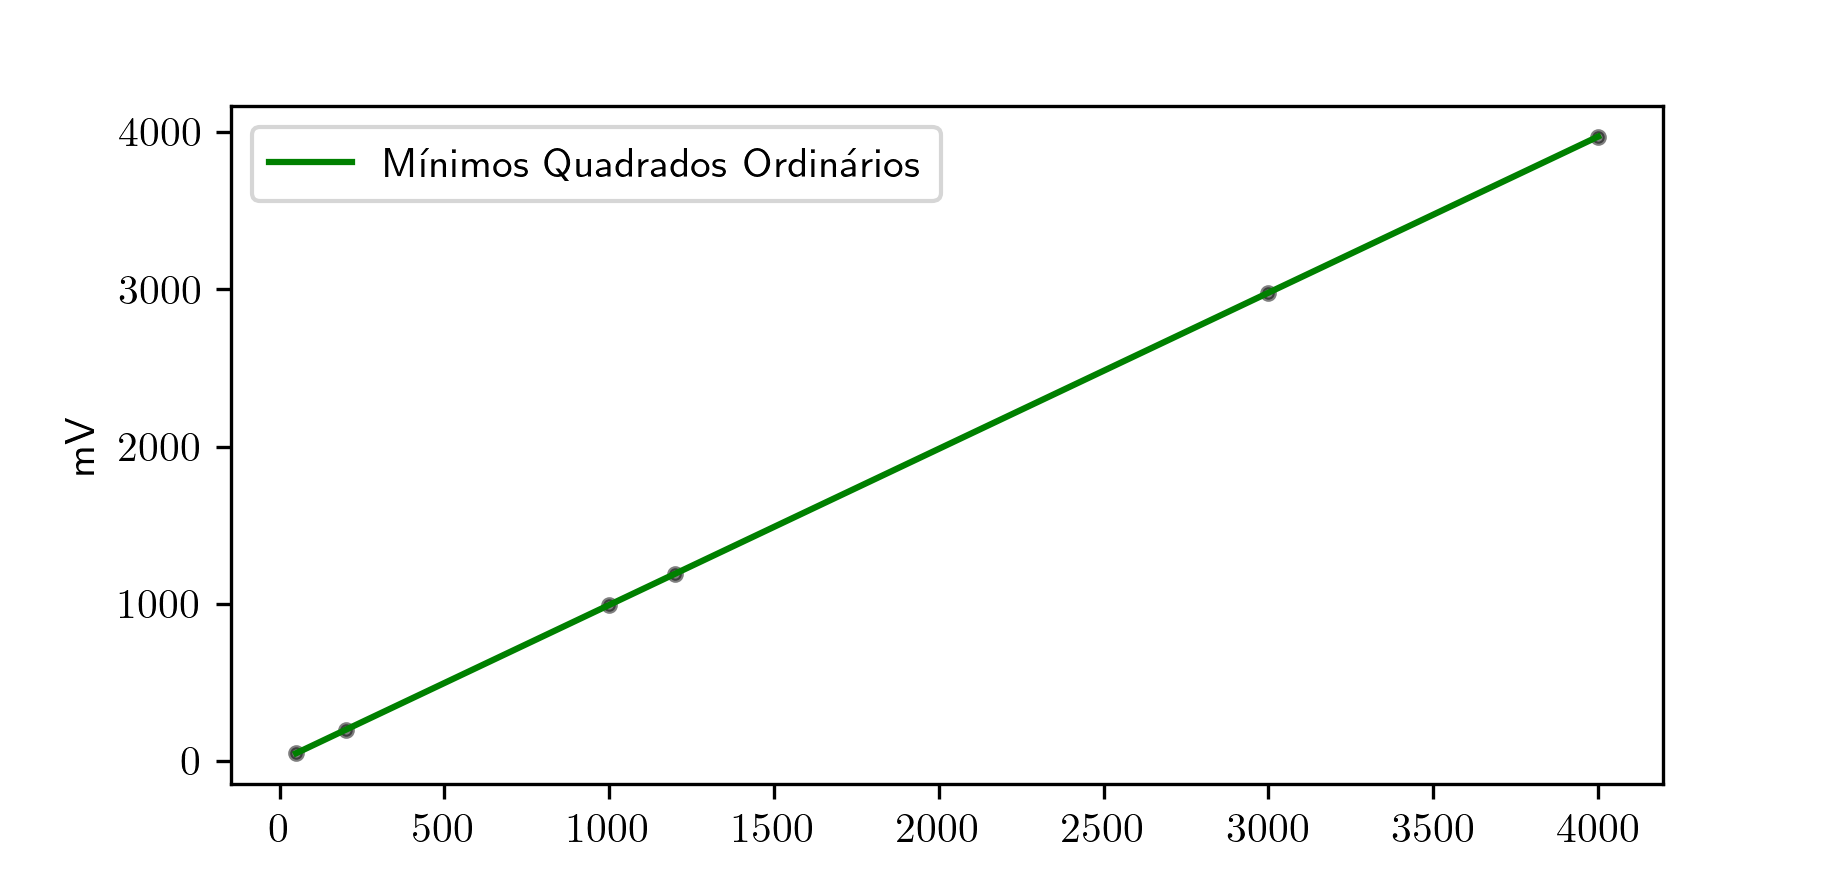
\includegraphics[width=12cm]{pictures/mqo_linha.png}
    \caption{Reta ajustada utilizando o método de Mínimos Quadrados Ordinários utilizando como sinais de entrada os valores RMS com maior erro em relação ao sinal aplicado para o canal IA}
    \label{fig:ols_line}
\end{figure}


\begin{table}[H]
\IBGEtab{%
  \caption[Sinais de corrente em 60Hz corrigidos após calibração utilizando Mínimos Quadrados Ordinários]{Sinais de corrente em 60Hz corrigidos após calibração utilizando Mínimos Quadrados Ordinários.}%
  \label{tab:tabelaerros60Aols}
} & \textbf{Valor Mín.} & \textbf{\%} & \textbf{Valor Méd.} & \textbf{\%}  \\
  \midrule
  50 & 0.6 \% & 50.0732 & 0.1464 & 49.9873 & -0.0254 & 50.6492 & 1.2984 \\
  \midrule
  200 & 0.2 \% & 199.9676 &	-0.0162 &	199.3803 &	-0.3098 & 200.2772 & 0.1386  \\
  \midrule
  1000 & 0.1 \% & 999.9097 & -0.009 & 996.6468 & -0.3353 & 1001.046 & 0.1046\\
  \midrule
  1200 & 0.1 \% & 1200.1783 & 0.0149 & 1196.2456 &	-0.3129 & 1201.7803 &	0.1484 \\
  \midrule
  3000 & 0.1 \% & 2999.8235 & -0.0059 & 2989.8713 &	-0.3376 & 2999.6535 &	-0.0116 \\
  \midrule
  4000 & 0.1 \% & 4000.1375 & 0.0034 & 3986.8394 &	-0.3290 & 4001.2924 &	0.0323 \\
  \bottomrule
\end{tabular}%
}{%
  \fonte{Produzido pelo autor.}%
 % \nota{rd representa o valor lido (em V).}
  %\nota{Esta é uma nota, que diz que os dados são baseados na
 % regressão linear. -- \showfont}%
  %\nota[Anotações]{Uma anotação adicional, que pode ser seguida de várias
  %outras. -- \showfont}%
  }
\end{table}


\begin{table}[H]
\IBGEtab{%
  \caption[Sinais de tensão em 60Hz corrigidos após calibração utilizando Mínimos Quadrados Ordinários]{Sinais de tensão em 60Hz corrigidos após calibração utilizando Mínimos Quadrados Ordinários.}%
  \label{tab:tabelaerros60Vols}
} & \textbf{Valor Mín.} & \textbf{\%} & \textbf{Valor Méd.} & \textbf{\%} \\
  \midrule
  9.2 & 0.1 \% & 9.3749 & 1.9014 & 9.4092 & 2.274 & 9.3173 & 1.8123\\
  \midrule
  57 & 0.1 \% & 57.7436 & 1.3046 & 57.6445 & 1.1307 & 57.7222 & 1.267   \\
  \midrule
  92 & 0.1 \% & 92.2785 & 0.3028 & 92.3173 & 0.3449 & 92.3547 & 0.3855 \\
  \midrule
  115 & 0.1 \% & 115.3321 & 0.2888 & 115.3641 & 0.3166 & 115.4533 & 0.3942 \\
  \midrule
  138 & 0.1 \% & 138.3352 &	0.2429 & 138.2648 &	0.1919 & 138.3077 &	0.2230 \\
  \midrule
  161 & 0.1 \% & 161.3615 & 0.2245 & 161.3868 &	0.2402 & 161.3902 &	0.2423\\
  \bottomrule
\end{tabular}%
}{%
  \fonte{Produzido pelo autor.}%
 % \nota{rd representa o valor lido (em V).}
  %\nota{Esta é uma nota, que diz que os dados são baseados na
 % regressão linear. -- \showfont}%
  %\nota[Anotações]{Uma anotação adicional, que pode ser seguida de várias
  %outras. -- \showfont}%
  }
\end{table}

Como é possível observar na tabela \ref{tab:tabelaerros60Aols}, houve significativa melhora nos erros relativos aos sinais de corrente. Após a calibração utilizando os pontos de erro máximo, os valores lidos em toda a faixa de aquisição passaram a se encontrar dentro da tolerância do equipamento. Entretanto, é perceptível que a calibração utilizando os pontos de erro mínimo e erro médio acabou por gerar coeficientes que, na maioria dos pontos, não reduziram tanto os erros quanto a calibração feita utilizando os pontos de erro máximo. Apesar disto, mesmo nestes casos as leituras ficaram dentro das especificações.

Já para os dados de tensão expostos na tabela \ref{tab:tabelaerros60Vols}, apesar da diminuição nos erros em toda a faixa de aquisição, estes ainda não se encontram dentro do especificado pelo fabricante (0.1 \% de 0.08Vn até 2Vn) em nenhum dos conjuntos de dados usados para calibração.

Com sinais aplicados com 50Hz, obtém-se os valores expostos nas tabelas \ref{tab:tabelaerros50Aols} e \ref{tab:tabelaerros50Vols} após a correção utilizando os coeficientes de primeira ordem utilizando o método de mínimos quadrados ordinários.

\begin{table}[H]
\IBGEtab{%
  \caption[Sinais de corrente em 50Hz corrigidos após calibração utilizando Mínimos Quadrados Ordinários]{Sinais de corrente em 50Hz corrigidos após calibração utilizando Mínimos Quadrados Ordinários.}%
  \label{tab:tabelaerros50Aols}
} & \textbf{Valor Mín.} & \textbf{\%} & \textbf{Valor Méd.} & \textbf{\%}  \\
  \midrule
  50 & 0.6 \% & 50.3303 & 0.6606 & 50.4465 & 0.893 & 49.6527 & -0.6947 \\
  \midrule
  200 & 0.2 \% & 199.8804 & -0.0598 & 200.5212 & 0.2606 & 199.4184 & -0.2908  \\
  \midrule
  1000 & 0.1 \% & 999.6978 & -0.0302 & 1001.8729 & 0.1873 & 1000.1444 & 0.0144\\
  \midrule
  1200 & 0.1 \% & 1200.0672 & 0.0056 & 1199.4922 & -0.0423 & 1197.7319 & -0.189 \\
  \midrule
  3000 & 0.1 \% & 2999.7407 & -0.0086 & 3002.3547 & 0.0785 & 2994.7691 & -0.1744 \\
  \midrule
  4000 & 0.1 \% & 4000.231 & 0.0058 & 4006.1437 & 0.1536 & 4002.1524 & 0.0538 \\
  \bottomrule
\end{tabular}%
}{%
  \fonte{Produzido pelo autor.}%
 % \nota{rd representa o valor lido (em V).}
  %\nota{Esta é uma nota, que diz que os dados são baseados na
 % regressão linear. -- \showfont}%
  %\nota[Anotações]{Uma anotação adicional, que pode ser seguida de várias
  %outras. -- \showfont}%
  }
\end{table}

\begin{table}[H]
\IBGEtab{%
  \caption[Sinais de tensão em 50Hz corrigidos após calibração utilizando Mínimos Quadrados Ordinários]{Sinais de tensão em 50Hz corrigidos após calibração utilizando Mínimos Quadrados Ordinários.}%
  \label{tab:tabelaerros50Vols}
} & \textbf{Valor Mín.} & \textbf{\%} & \textbf{Valor Méd.} & \textbf{\%} \\
  \midrule
  9.2 & 0.1 \% & 9.5037 & 3.3011 & 10.2354 & 11.2543 & 9.3615 & 1.7554\\
  \midrule
  57 & 0.1 \% & 57.7989 & 1.4015 & 61.4752 & 7.8512 & 57.6901 & 1.2107\\
  \midrule
  92 & 0.1 \% & 92.3592 & 0.3904 & 109.4042 & 18.9176 & 92.3574 & 0.3885\\
  \midrule
  115 & 0.1 \% & 115.3925 & 0.3413 & 135.9996 & 18.2605 & 115.1646 & 0.1431 \\
  \midrule
  138 & 0.1 \% & 138.4393 & 0.3184 & 140.8817 & 2.0882 & 138.1461 & 0.1059 \\
  \midrule
  161 & 0.1 \% & 161.4813 & 0.299 & 163.7498 & 1.7079 & 161.4896 & 0.3041\\
  \bottomrule
\end{tabular}%
}{%
  \fonte{Produzido pelo autor.}%
 % \nota{rd representa o valor lido (em V).}
  %\nota{Esta é uma nota, que diz que os dados são baseados na
 % regressão linear. -- \showfont}%
  %\nota[Anotações]{Uma anotação adicional, que pode ser seguida de várias
  %outras. -- \showfont}%
  }
\end{table}

Analisando os resultados para sinais de corrente, é perceptível que o único ponto a estar fora das especificações do fabricante (0.6 $\%$) possui 50 mA de amplitude, tanto utilizando como valores de entrada os valores RMS dos ciclos com maior erro em relação ao valor aplicado, quanto utilizando os valores RMS com erro mínimo por ciclo ou o valor médio entre os valores RMS obtidos em todos os ciclos de aquisição.  Para sinais de corrente com amplitude maior, a calibração mostrou-se suficiente. Nos resultados para sinais de tensão, observa-se um erro máximo superando os 0.1 $\%$ máximos segundo o fabricante para toda a extensão de valores aplicados, tanto utilizando como valores de entrada os valores RMS com maior erro em relação ao valor aplicado quanto os valores com menor, bem como o erro entre o valor RMS médio entre todos os ciclos de sinal capturados. 

A tabela \ref{tab:tabelaerros60olsrsq} expõe os valores de $R^2$ para cada um dos conjuntos de dados usados para a linearização. É observável que, uma vez que a linearização traz resultados muito próximos dos nominais, este valor é muito próximo de 1. Entretanto, como critério de avaliação, o coeficiente $R^2$ traz poucas informações, pois para todos os valores de entrada este coeficiente torna-se muito próximo de 1.

\begin{table}[H]
\IBGEtab{%
  \caption[Coeficientes $R^2$ para a linearização por Mínimos Quadrados Ordinários]{Coeficientes $R^2$ para a linearização por Mínimos Quadrados Ordinários.}%
  \label{tab:tabelaerros60olsrsq}
}{%
  \begin{tabular}{ccc}
  \toprule
   & \textbf{Canal IA} &  \\
  \midrule
 \textbf{$R^2$ Erro máximo} & \textbf{ $R^2$ Erro Mínimo} & \textbf{$R^2$ Erro médio}   \\
  \midrule
  999999992454582 & 0.999999681815048 & 0.99999977198064\\
    \toprule
    & \textbf{Canal VC} & \\
     \midrule
 \textbf{$R^2$ Erro máximo} & \textbf{ $R^2$ Erro Mínimo} & \textbf{$R^2$ Erro médio}   \\
    \midrule
  0.999987761633336 & 0.999992528523623 & 0.999990248990353\\
    \bottomrule
\end{tabular}%
}{%
  \fonte{Produzido pelo autor.}%
 % \nota{rd representa o valor lido (em V).}
  %\nota{Esta é uma nota, que diz que os dados são baseados na
 % regressão linear. -- \showfont}%
  %\nota[Anotações]{Uma anotação adicional, que pode ser seguida de várias
  %outras. -- \showfont}%
  }
\end{table}


\section{Mínimos Quadrados Ponderados}

Já utilizando o método dos mínimos quadrados ponderados, os resultados da calibração estão expostos nas tabelas \ref{tab:tabelaerros60Awls} para corrente e \ref{tab:tabelaerros60Vwls} para tensão. É digno de menção que o vetor de a matriz diagonal de pesos utilizada é inversamente proporcional aos erros máximos especificados pelo fabricante nas tabelas \ref{tab:specsMEA} e \ref{tab:specsMEV}, isto é: os sinais aplicados em regiões de aquisição com erro menor permitido terão peso maior na linearização. A figura \ref{fig:wls_line} ilustra a reta ajustada após a aplicação deste método.

\begin{figure}[H]
    \centering
    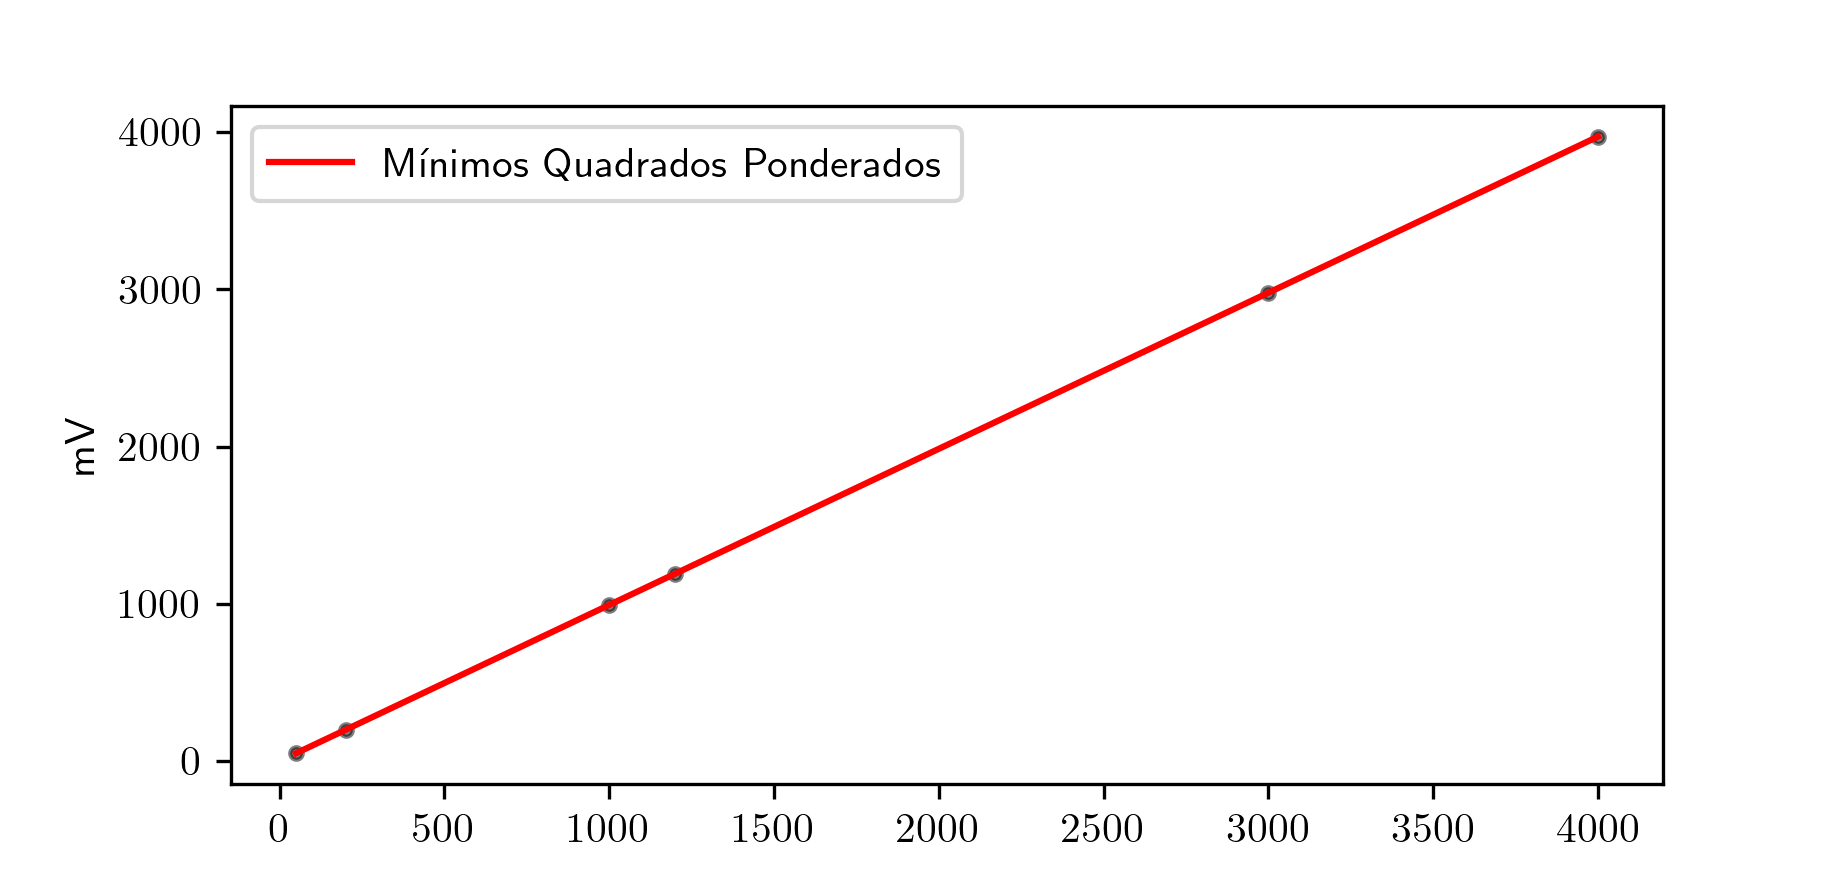
\includegraphics[width=12cm]{pictures/mqp_linha.png}
    \caption{Reta ajustada utilizando o método de Mínimos Quadrados Ponderados utilizando como sinais de entrada os valores RMS com maior erro em relação ao sinal aplicado para o canal IA}
    \label{fig:wls_line}
\end{figure}

\begin{table}[H]
\IBGEtab{%
  \caption[Sinais de corrente com frequência de 60Hz corrigidos após calibração utilizando Mínimos Quadrados Ponderados]{[Sinais de corrente com frequência de 60Hz corrigidos após calibração utilizando Mínimos Quadrados Ponderados.}%
  \label{tab:tabelaerros60Awls}
} & \textbf{Valor Mín.} & \textbf{\%} & \textbf{Valor Méd.} & \textbf{\%} \\
  \midrule
  50 & 0.6 \% & 50.0988 & 0.1976 & 50.7535 & 1.507 & 51.0945	& 2.1889\\
  \midrule
  200 & 0.2 \% & 199.9982 & -0.0009 & 200.1686 & 0.0843 & 200.7633 & 0.3816\\
  \midrule
  1000 & 0.1 \% & 999.9671 & -0.0033 & 1001.1913 & 0.1191 & 1001.7502 & 0.175\\
  \midrule
  1200 & 0.1 \% & 1200.2424 & 0.0202 & 1201.5306 & 0.1275 & 1202.5392 & 0.2116\\
  \midrule
  3000 & 0.1 \% & 2999.9478 & -0.0017 & 2999.9857 & -0.0005 & 3000.9022 & 0.0301\\
  \midrule
  4000 & 0.1 \% & 4000.2953 & 0.0074 & 4002.8304 & 0.0708 & 4002.814 & 0.0704\\
  \bottomrule
\end{tabular}%
}{%
  \fonte{Produzido pelo autor.}%
 % \nota{rd representa o valor lido (em V).}
  %\nota{Esta é uma nota, que diz que os dados são baseados na
 % regressão linear. -- \showfont}%
  %\nota[Anotações]{Uma anotação adicional, que pode ser seguida de várias
  %outras. -- \showfont}%
  }
\end{table}

\begin{table}[H]
\IBGEtab{%
  \caption[Sinais de tensão com frequência de 60Hz corrigidos após calibração utilizando Mínimos Quadrados Ponderados]{Sinais de tensão com frequência de 60Hz corrigidos após calibração utilizando Mínimos Quadrados Ponderados.}%
  \label{tab:tabelaerros60Vwls}
} & \textbf{Valor Mín.} & \textbf{\%} & \textbf{Valor Méd.} & \textbf{\%} \\
  \midrule
  9.2 & 0.1 \% &  9.3749 & 1.9014 & 9.4092 & 2.274 & 9.4173 & 2.3623\\
  \midrule
  57 & 0.1 \% & 57.7436 & 1.3046 & 57.6445 & 1.1307 & 57.7222 & 1.267\\
  \midrule
  92 & 0.1 \% & 92.2785 & 0.3028 & 92.3173 & 0.3449 & 92.3547 & 0.3855\\
  \midrule
  115 & 0.1 \% & 115.3321 & 0.2888 & 115.3641 & 0.3166 & 115.4533 & 0.3942 \\
  \midrule
  138 & 0.1 \% & 138.3352 & 0.2429 & 138.2648 & 0.1919 & 138.3077 & 0.223\\
  \midrule
  161 & 0.1 \% & 161.3615 & 0.2245 & 161.3868 & 0.2402 & 161.3902 & 0.2423\\
  \bottomrule
\end{tabular}%
}{%
  \fonte{Produzido pelo autor.}%
 % \nota{rd representa o valor lido (em V).}
  %\nota{Esta é uma nota, que diz que os dados são baseados na
 % regressão linear. -- \showfont}%
  %\nota[Anotações]{Uma anotação adicional, que pode ser seguida de várias
  %outras. -- \showfont}%
  }
\end{table}

Da mesma forma que no método anterior, é possível verificar que a calibração do canal de tensão mostrou-se insuficiente para trazer a leitura dos sinais de tensão para dentro das especificações do equipamento, tendo como piores casos os sinais com amplitude menor. Para o canal de corrente, são observados resultados semelhantes utilizando os pontos com erro máximo como entrada do algoritmo. Entretanto, utilizando os pontos de erro mínimo e de erro médio, a linearização acabou piorando o erro nos pontos com menor amplitude de corrente, sendo suficiente para não atender as especificações.

Utilizando os sinais de 50Hz como entrada do método, obtém-se as tabelas \ref{tab:tabelaerros50Awls} \ref{tab:tabelaerros50Vwls} após aplicação dos coeficientes gerados para correção.

Com  este método, foram obtidos resultados dentro dos máximos permitidos pelo fabricante para toda a faixa de aquisição de corrente utilizando como valores de entrada os valores RMS com erro máximo entre os ciclos e erro médio entre todos os ciclos RMS. Utilizando o erro mínimo por ciclo como entrada para o método, o sinal de 50mA permanece fora das especificações do fabricante.

Para as aquisições de tensão, em nenhum dos grupos de sinais de entrada foi possível atingir os mínimos descritos na documentação do equipamento (0.1 \%).

\begin{table}[H]
\IBGEtab{%
  \caption[Sinais de corrente com frequência de 50Hz corrigidos após calibração utilizando Mínimos Quadrados Ponderados]{Sinais de corrente com frequência de 50Hz corrigidos após calibração utilizando Mínimos Quadrados Ponderados.}%
  \label{tab:tabelaerros50Awls}
} & \textbf{Valor Mín.} & \textbf{\%} & \textbf{Valor Méd.} & \textbf{\%} \\
  \midrule
  50 & 0.6 \% & 50.2551 & 0.5102 & 57.6585 & 15.3169 & 50.2479 & 0.4957\\
  \midrule
  200 & 0.2 \% & 199.8071 & -0.0965 & 199.6745 & -0.1627 & 200.0427 & 0.0213\\
  \midrule
  1000 & 0.1 \% & 999.6346 & -0.0365 & 999.3963 & -0.0604 & 1001.5594 & 0.1559\\
  \midrule
  1200 & 0.1 \% & 1200.0065 & 0.0005 & 1196.9341 & -0.2555 & 1199.3174 & -0.0569\\
  \midrule
  3000 & 0.1 \% & 2999.7027 & -0.0099 & 2999.0531 & -0.0316 & 2997.9047 & -0.0698\\
  \midrule
  4000 & 0.1 \% & 4000.2057 & 0.0051 & 4002.4282 & 0.0607 & 4006.1568 & 0.1539\\
  \bottomrule
\end{tabular}%
}{%
  \fonte{Produzido pelo autor.}%
 % \nota{rd representa o valor lido (em V).}
  %\nota{Esta é uma nota, que diz que os dados são baseados na
 % regressão linear. -- \showfont}%
  %\nota[Anotações]{Uma anotação adicional, que pode ser seguida de várias
  %outras. -- \showfont}%
  }
\end{table}

\begin{table}[H]
\IBGEtab{%
  \caption[Sinais de tensão com frequência de 50Hz corrigidos após calibração utilizando Mínimos Quadrados Ponderados]{Sinais de tensão com frequência de 50Hz corrigidos após calibração utilizando Mínimos Quadrados Ponderados.}%
  \label{tab:tabelaerros50Vwls}
} & \textbf{Valor Mín.} & \textbf{\%} & \textbf{Valor Méd.} & \textbf{\%} \\
  \midrule
  9.2 & 0.1 \% & 9.3749 & 1.9014 & 9.4092 & 2.274 & 9.4173 & 2.3623\\
  \midrule
  57 & 0.1 \% & 57.7436 & 1.3046 & 57.6445 & 1.1307 & 57.7222 & 1.267\\
  \midrule
  92 & 0.1 \% & 92.2785 & 0.3028 & 92.3173 & 0.3449 & 92.3547 & 0.3855\\
  \midrule
  115 & 0.1 \% & 115.3321 & 0.2888 & 115.3641 & 0.3166 & 115.4533 & 0.3942 \\
  \midrule
  138 &  0.1 \% & 138.3352 & 0.2429 & 138.2648 & 0.1919 & 138.3077 & 0.223\\
  \midrule
  161 & 0.1 \% & 161.3615 & 0.2245 & 161.3868 & 0.2402 & 161.3902 & 0.2423\\
  \bottomrule
\end{tabular}%
}{%
  \fonte{Produzido pelo autor.}%
 % \nota{rd representa o valor lido (em V).}
  %\nota{Esta é uma nota, que diz que os dados são baseados na
 % regressão linear. -- \showfont}%
  %\nota[Anotações]{Uma anotação adicional, que pode ser seguida de várias
  %outras. -- \showfont}%
  }
\end{table}

Da mesma forma que no método de mínimos quadrados ordinários, os coeficientes de determinação  $R^2$ não trazem informações muito úteis na análise, exceto por descrever a boa linearização obtida pelo algoritmo. A tabela \ref{tab:tabelaerros60wlsrsq} expõe estes valores.

\begin{table}[H]
\IBGEtab{%
  \caption[Coeficientes $R^2$ para a linearização por Mínimos Quadrados Ponderados]{Coeficientes $R^2$ para a linearização por Mínimos Quadrados Ponderados.}%
  \label{tab:tabelaerros60wlsrsq}
}{%
  \begin{tabular}{ccc}
  \toprule
   & \textbf{Canal IA} &\\
  \midrule
 \textbf{$R^2$ Erro máximo} & \textbf{ $R^2$ Erro Mínimo} & \textbf{$R^2$ Erro médio}   \\
  \midrule
 0.999999900283003 & 0.99999952000389 & 0.99999960002109\\
    \toprule
   &  \textbf{Canal VC} &  \\
     \midrule
 \textbf{$R^2$ Erro máximo} & \textbf{ $R^2$ Erro Mínimo} & \textbf{$R^2$ Erro médio}   \\
    \midrule
0.9999835900083 & 0.99999036982379 & 0.999987420008623\\
    \bottomrule
\end{tabular}%
}{%
  \fonte{Produzido pelo autor.}%
 % \nota{rd representa o valor lido (em V).}
  %\nota{Esta é uma nota, que diz que os dados são baseados na
 % regressão linear. -- \showfont}%
  %\nota[Anotações]{Uma anotação adicional, que pode ser seguida de várias
  %outras. -- \showfont}%
  }
\end{table}

\section{Mínimos Desvios Absolutos}

Corrigindo os valores expostos nas tabelas \ref{tab:specsMEA} e \ref{tab:specsMEV} com os coeficientes de primeira ordem resultantes da aplicação do método de mínimos desvios absolutos, são obtidos os resultados expostos nas tabelas \ref{tab:tabelaerros60Alad} e \ref{tab:tabelaerros60Vlad}. A figura \ref{fig:lad_line} ilustra a reta ajustada após a aplicação deste método.

\begin{figure}[H]
    \centering
    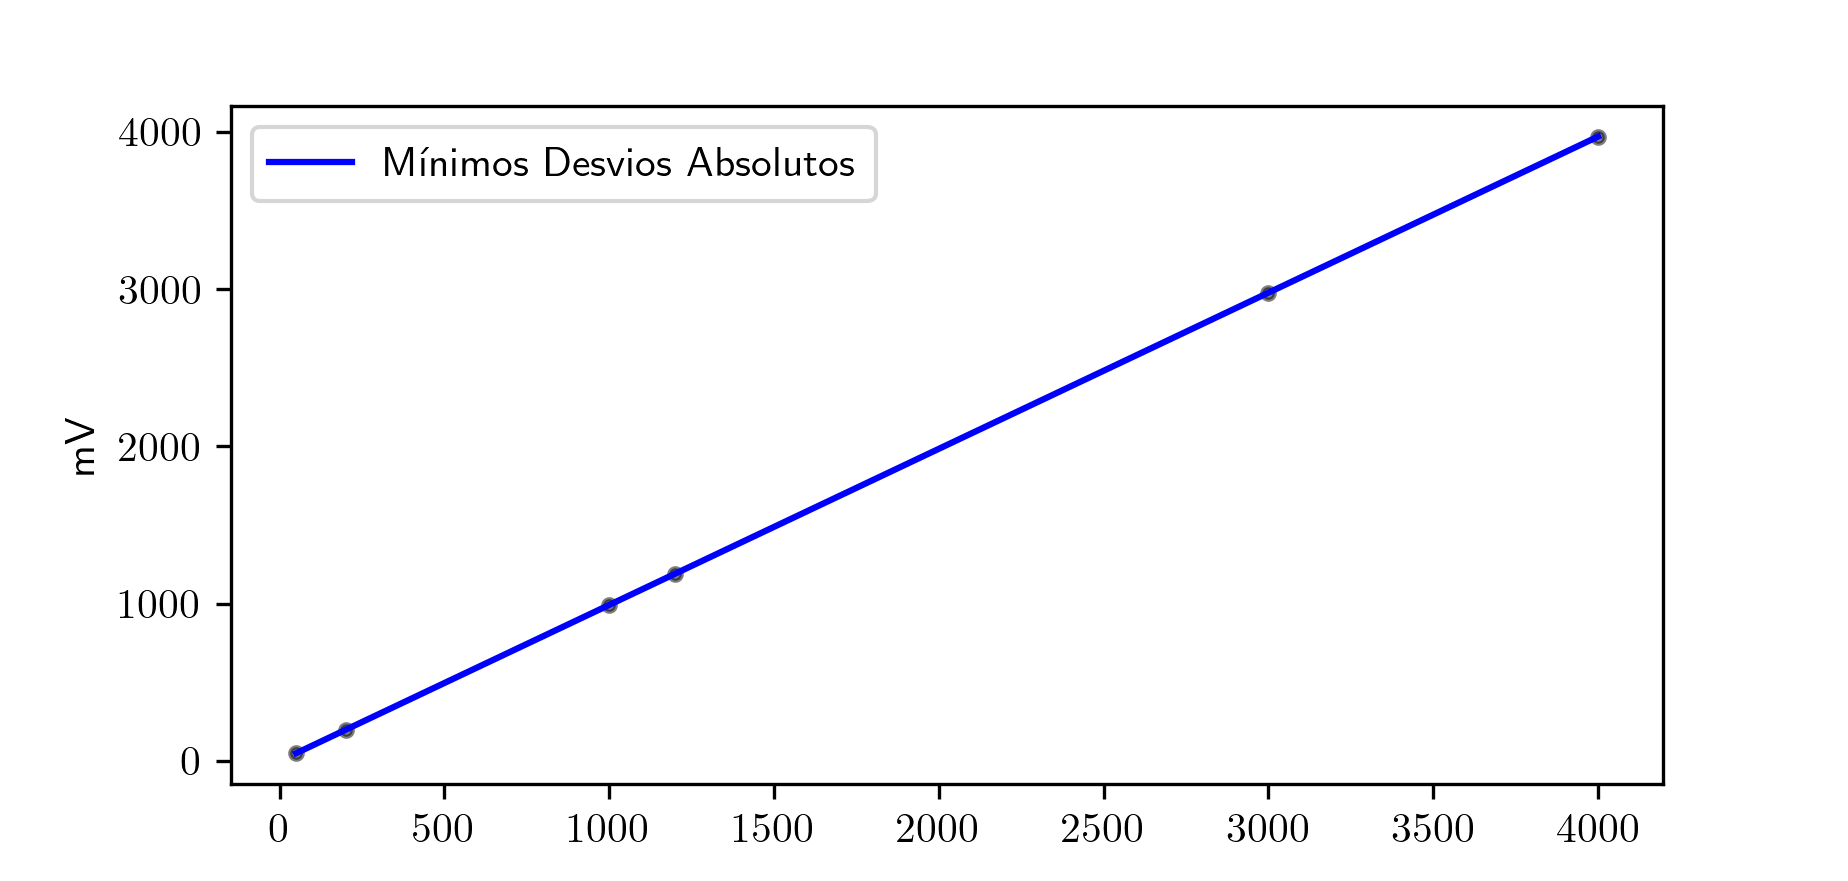
\includegraphics[width=12cm]{pictures/mda_linha.png}
    \caption{Reta ajustada utilizando o método de Mínimos Desvios Absolutos utilizando como sinais de entrada os valores RMS com maior erro em relação ao sinal aplicado para o canal IA}
    \label{fig:lad_line}
\end{figure}

\begin{table}[H]
\IBGEtab{%
  \caption[Sinais de corrente com 60Hz corrigidos após calibração utilizando Mínimos Desvios Absolutos]{Sinais de corrente corrigidos após calibração utilizando Mínimos Desvios Absolutos.}%
  \label{tab:tabelaerros60Alad}
} & \textbf{Valor Mín.} & \textbf{\%} & \textbf{Valor Méd.} & \textbf{\%} \\
  \midrule
  50 & 0.6 \% & 50.015 & 0.0299 & 50.4466 & 0.8932 & 50.8247 & 1.6494\\
  \midrule
  200 & 0.2 \% & 199.9026 & -0.0487 & 199.7801 & -0.1099 & 200.4405 & 0.2202\\
  \midrule
  1000 & 0.1 \% & 999.809 & -0.0191 & 1000.3653 & 0.0365 & 1001.1435 & 0.1143\\
  \midrule
  1200 & 0.1 \% & 1200.0687 &  0.0057 & 1200.5952 & 0.0496 & 1201.8613 & 0.1551\\
  \midrule
  3000 & 0.1 \% & 2999.6333 & -0.0122 & 2998.0683 & -0.0644 & 2999.5868 & -0.0138 \\
  \midrule
  4000 & 0.1 \% & 3999.9026 & -0.0024 & 4000.3653 & 0.0091 & 4001.1435 & 0.0286\\
  \bottomrule
\end{tabular}%
}{%
  \fonte{Produzido pelo autor.}%
 % \nota{rd representa o valor lido (em V).}
  %\nota{Esta é uma nota, que diz que os dados são baseados na
 % regressão linear. -- \showfont}%
  %\nota[Anotações]{Uma anotação adicional, que pode ser seguida de várias
  %outras. -- \showfont}%
  }
\end{table}

\begin{table}[H]
\IBGEtab{%
  \caption[Sinais de tensão com 60Hz corrigidos após calibração utilizando Mínimos Desvios Absolutos]{Sinais de tensão corrigidos após calibração utilizando Mínimos Desvios Absolutos.}%
  \label{tab:tabelaerros60Vlad}
} & \textbf{Valor Mín.} & \textbf{\%} & \textbf{Valor Méd.} & \textbf{\%} \\
  \midrule
  9.2 & 0.1 \% & 9.3201 &	1.3055 &	9.939 &	8.0331 & 10.0301 & 9.0226\\
  \midrule
  57 & 0.1 \% & 57.6822 & 1.1969 & 58.3836 & 2.4274 & 58.5599 & 2.7367\\
  \midrule
  92 & 0.1 \% & 92.2125 & 0.2309 & 93.2068 & 1.3118 & 93.3537 & 1.4714\\
  \midrule
  115 & 0.1 \% & 115.2629 & 0.2286 & 116.3537 & 1.1771 & 116.5599 & 1.3564\\
  \midrule
  138 & 0.1 \% & 138.2629 & 0.1905 & 139.3537 & 0.9809 & 139.5208 & 1.102\\
  \midrule
  161 & 0.1 \% & 161.2861 & 0.1777 & 162.576 & 0.9789 & 162.7107 & 1.0625\\
  \bottomrule
\end{tabular}%
}{%
  \fonte{Produzido pelo autor.}%
 % \nota{rd representa o valor lido (em V).}
  %\nota{Esta é uma nota, que diz que os dados são baseados na
 % regressão linear. -- \showfont}%
  %\nota[Anotações]{Uma anotação adicional, que pode ser seguida de várias
  %outras. -- \showfont}%
  }
\end{table}

Utilizando o método dos Mínimos Desvios Absolutos com sinais com frequência de 60 Hz, a linearização à partir dos pontos de maior erro em relação à amplitude dos sinais de corrente aplicados trouxe resultados melhores que nos dois métodos anteriores para os pontos máximo e mínimo. Para valores mais próximos do nominal, este método teve resultados semelhantes aos dois métodos anteriores. Da mesma forma que os dois métodos anteriores, a calibração utilizando os pontos de erro mínimo e erro médio trouxeram resultados insuficientes para fazer com que o erro fique dentro das suas próprias especificações.

Com sinais de entrada com frequência de 50 Hz, os resultados estão expostos nas tabelas \ref{tab:tabelaerros50Alad} e \ref{tab:tabelaerros50Vlad}.

\begin{table}[H]
\IBGEtab{%
  \caption[Sinais de corrente com 50Hz corrigidos após calibração utilizando Mínimos Desvios Absolutos]{Sinais de corrente corrigidos após calibração utilizando Mínimos Desvios Absolutos.}%
  \label{tab:tabelaerros50Alad}
} & \textbf{Valor Mín.} & \textbf{\%} & \textbf{Valor Méd.} & \textbf{\%} \\
  \midrule
  50 & 0.6 \% & 50.2083 & 0.4167 & 57.7874 & 15.5748 & 49.8114 & -0.3772\\
  \midrule
  200 & 0.2 \% & 199.7446 & -0.1277 & 199.8041 & -0.098 & 199.3656 & -0.3172\\
  \midrule
  1000 & 0.1 \% & 999.4883 & -0.0512 & 999.5293 & -0.0471 & 999.5949 & -0.0405\\
  \midrule
  1200 & 0.1 \% & 1199.8391 & -0.0134 & 1197.068 & -0.2443 & 1197.0352 & -0.2471\\
  \midrule
  3000 & 0.1 \% & 2999.3466 & -0.0218 & 2999.1949 & -0.0268 & 2992.7333 & -0.2422 \\
  \midrule
  4000 & 0.1 \% & 3999.7447 & -0.0064 & 4002.5744 & 0.0644 & 3999.3659 & -0.0159\\
  \bottomrule
\end{tabular}%
}{%
  \fonte{Produzido pelo autor.}%
 % \nota{rd representa o valor lido (em V).}
  %\nota{Esta é uma nota, que diz que os dados são baseados na
 % regressão linear. -- \showfont}%
  %\nota[Anotações]{Uma anotação adicional, que pode ser seguida de várias
  %outras. -- \showfont}%
  }
\end{table}

\begin{table}[H]
\IBGEtab{%
  \caption[Sinais de tensão com 50Hz corrigidos após calibração utilizando Mínimos Desvios Absolutos]{Sinais de tensão corrigidos após calibração utilizando Mínimos Desvios Absolutos.}%
  \label{tab:tabelaerros50Vlad}
} & \textbf{Valor Mín.} & \textbf{\%} & \textbf{Valor Méd.} & \textbf{\%} \\
  \midrule
  9.2 & 0.1 \% & 9.2509 & 0.5532 & 11.7113 & 27.2963 & 9.8202 & 6.7416\\
  \midrule
  57 & 0.1 \% & 57.4621 & 0.8107 & 59.1408 & 3.7559 & 58.3718 & 2.4067\\
  \midrule
  92 & 0.1 \% & 91.9623 & -0.0409 & 107.8784 & 17.2592 & 93.1991 & 1.3034\\
  \midrule
  115 & 0.1 \% & 114.9556 & -0.0386 & 134.9226 & 17.324 & 116.1116 & 0.9666\\
  \midrule
  138 & 0.1 \% & 137.9624 & -0.0273 & 139.887 & 1.3674 & 139.1992 & 0.869\\
  \midrule
  161 & 0.1 \% & 160.9643 & -0.0222 & 163.1409 & 1.3297 & 162.6504 & 1.0251\\
  \bottomrule
\end{tabular}%
}{%
  \fonte{Produzido pelo autor.}%
 % \nota{rd representa o valor lido (em V).}
  %\nota{Esta é uma nota, que diz que os dados são baseados na
 % regressão linear. -- \showfont}%
  %\nota[Anotações]{Uma anotação adicional, que pode ser seguida de várias
  %outras. -- \showfont}%
  }
\end{table}

No caso da calibração do canal de tensão, nem mesmo para os pontos de erro máximo são obtidos resultados satisfatórios. A não-linearidade dos pontos é tão grande nesse canal que nem mesmo para os sinais com maior amplitude o erro é baixo o suficiente para atingir as especificações do fabricante.

\section{Análise dos Resultados}

Com o intuito de avaliar os resultados dos três métodos de maneira simultânea, o gráfico da \figref{fig:res_curr} expõe a porcentagem do erro máximo trazido pelo fabricante que os sinais de corrente possuem após as calibrações utilizando sinais de 60Hz. 

\begin{figure}[H]
    \caption{Porcentagem do erro máximo atingido para os sinais de corrente com maior erro por ciclo após a aplicação do Método dos Mínimos Quadrados Ordinários (MQO), do Método dos Mínimos Quadrados Ponderados (MQP) e do método dos Mínimos Desvios Absolutos (MDA) em 60 Hz}
    \label{fig:res_curr}
    \centering
    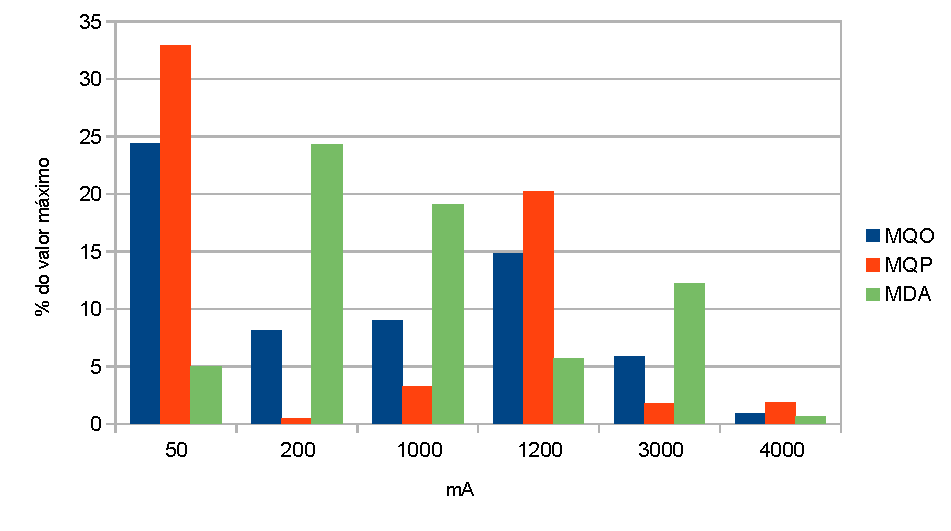
\includegraphics[width=0.9\linewidth]{pictures/max_err_IA_aftercalib60Hz}
    \fonte{o autor.}
\end{figure}

Com isto, é possível observar que o Método dos Mínimos Desvios Absolutos foi capaz de minimizar o erro mais do que os outros métodos para o sinal de menor amplitude. No entanto, para a maioria dos pontos seguintes, este método trouxe erros superiores aos outros, apesar de continuar mantendo-se dentro das especificações do fabricante. Já no Método dos Mínimos Quadrados Ordinários, os coeficientes obtidos geraram um maior erro para o ponto de menor amplitude, mas para os outros pontos este erro foi sempre menor que 15 \% do permitido. Por fim, o Método dos Mínimos Quadrados ponderados trouxe o pior erro para o sinal com amplitude mais baixa, mas exceto pelo ponto de 1.2A no qual o erro ultrapassou os 20\% do valor máximo fornecido pelo fabricante, o erro manteve-se menor que todos os outros métodos. De forma a resumir essa relação, a tabela \ref{tab:med_rescurr} expõe a média dos erros para o canal de aquisição de corrente analisado.

\begin{table}[H]
\IBGEtab{%
  \caption[Média dos erros em relação ao máximo permitido pelo fabricante para o canal de corrente IA em 60 Hz.]{Média dos erros em relação ao máximo permitido pelo fabricante para o canal de corrente IA em 60 Hz.}%
  \label{tab:med_rescurr}
}{%
  \begin{tabular}{ccc}
  \toprule
   & \textbf{Canal IA} & \\
  \midrule
  \textbf{Erro Médio MQO (\%)} & \textbf{Erro Médio MQP (\%)} & \textbf{Erro Médio MDA (\%)}  \\ 
  \midrule
  10.5228 &	10.0768 & 11.1635 \\
  \bottomrule
\end{tabular}%
}{%
  \fonte{Produzido pelo autor.}%
 % \nota{rd representa o valor lido (em V).}
  %\nota{Esta é uma nota, que diz que os dados são baseados na
 % regressão linear. -- \showfont}%
  %\nota[Anotações]{Uma anotação adicional, que pode ser seguida de várias
  %outras. -- \showfont}%
  }
\end{table}

Fazendo a mesma análise utilizando o canal de tensão VC, observa-se que em nenhum dos métodos os resultado foi suficiente para que as leituras possuam erros menores do que os erros máximos fornecidos pelo fabricante. A \figref{fig:res_volt} ilustra esse resultado. 

\begin{figure}[H]
    \caption{Porcentagem do erro máximo atingido para os sinais de tensão com maior erro por ciclo após a aplicação do Método dos Mínimos Quadrados Ordinários (MQO), do Método dos Mínimos Quadrados Ponderados (MQP) e do método dos Mínimos Desvios Absolutos (MDA).}
    \label{fig:res_volt}
    \centering
    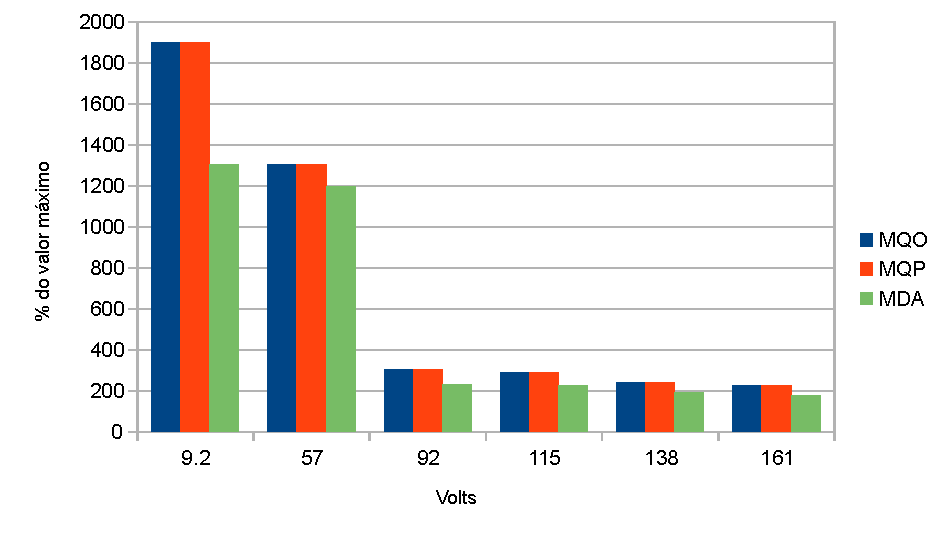
\includegraphics[width=0.9\linewidth]{pictures/max_err_VC_aftercalib60.pdf}
    \fonte{o autor.}
\end{figure}

A tabela \ref{tab:med_resvolt} expõe as médias dos erros obtidos nas três calibrações, em porcentagem do máximo permitido pelo fabricante.

\begin{table}[H]
\IBGEtab{%
  \caption[Média dos erros em relação ao máximo permitido pelo fabricante para o canal de tensão VC em 60 Hz.]{Média dos erros em relação ao máximo permitido pelo fabricante para o canal de tensão VC em 60 Hz.}%
  \label{tab:med_resvolt}
}{%
  \begin{tabular}{ccc}
  \toprule
   & \textbf{Canal VC}  & \\
  \midrule
  \textbf{Erro Médio MQO (\%)} & \textbf{Erro Médio MQP (\%)} & \textbf{Erro Médio MDA (\%)}  \\ 
  \midrule
  710.8315 & 710.8315 & 555.013 \\
  \bottomrule
\end{tabular}%
}{%
  \fonte{Produzido pelo autor.}%
 % \nota{rd representa o valor lido (em V).}
  %\nota{Esta é uma nota, que diz que os dados são baseados na
 % regressão linear. -- \showfont}%
  %\nota[Anotações]{Uma anotação adicional, que pode ser seguida de várias
  %outras. -- \showfont}%
  }
\end{table}

Da mesma forma, utilizando sinais de entrada de 50 Hz, temos os resultados expostos nas imagens \ref{fig:res_curr50} para corrente e \ref{fig:res_volt50} para tensão. No canal de corrente, os métodos de Mínimos Quadrados Ponderados e Mínimos Desvios Absolutos em primeira ordem são suficientes para compensar as leituras e deixar o equipamento dentro das especificações do fabricante. No método de Mínimos Quadrados Ordinários, o resultado mostra-se insuficiente para 50 mA. Já para o canal de tensão, da mesma forma que utilizando sinais de entrada com 60 Hz, nenhum dos três métodos é suficiente para a calibração em primeira ordem. As tabelas \ref{tab:med_rescurr} e \ref{tab:med_resvolt} expõem os erros médios após estas calibrações.


\begin{figure}[H]
    \caption{Porcentagem do erro máximo atingido para os sinais de corrente com maior erro por ciclo após a aplicação do Método dos Mínimos Quadrados Ordinários (MQO), do Método dos Mínimos Quadrados Ponderados (MQP) e do método dos Mínimos Desvios Absolutos (MDA) em 50 Hz}
    \label{fig:res_curr50}
    \centering
    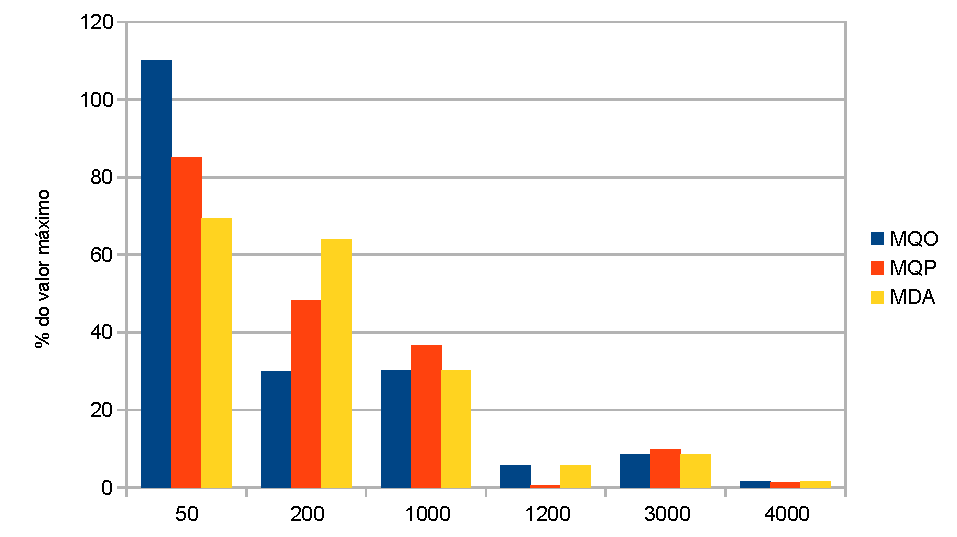
\includegraphics[width=0.9\linewidth]{pictures/max_err_IA_aftercalib50Hz.pdf}
    \fonte{o autor.}
\end{figure}

\begin{figure}[H]
    \caption{Porcentagem do erro máximo atingido para os sinais de tensão em 50 Hz com maior erro por ciclo após a aplicação do Método dos Mínimos Quadrados Ordinários (MQO), do Método dos Mínimos Quadrados Ponderados (MQP) e do método dos Mínimos Desvios Absolutos (MDA).}
    \label{fig:res_volt50}
    \centering
    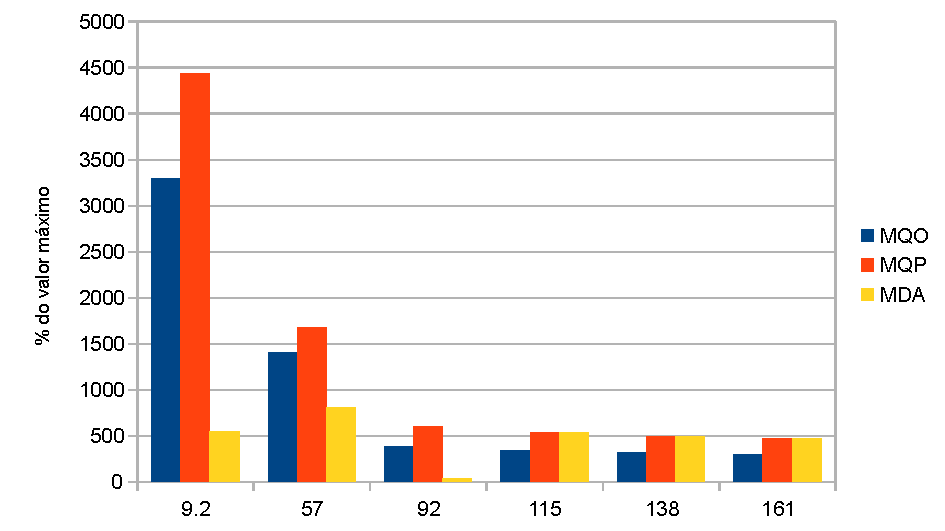
\includegraphics[width=0.9\linewidth]{pictures/max_err_VC_aftercalib50Hz.pdf}
    \fonte{o autor.}
\end{figure}

\begin{table}[H]
\IBGEtab{%
  \caption[Média dos erros em relação ao máximo permitido pelo fabricante para o canal de corrente IA em 50 Hz.]{Média dos erros em relação ao máximo permitido pelo fabricante para o canal de corrente IA em 50 Hz.}%
  \label{tab:med_rescurr50}
}{%
  \begin{tabular}{ccc}
  \toprule
   & \textbf{Canal IA} &  \\
  \midrule
  \textbf{Erro Médio MQO (\%)} & \textbf{Erro Médio MQP (\%)} & \textbf{Erro Médio MDA (\%)}  \\ 
  \midrule
  30.9858 &	30.258 & 29.8665 \\
  \bottomrule
\end{tabular}%
}{%
  \fonte{Produzido pelo autor.}%
 % \nota{rd representa o valor lido (em V).}
  %\nota{Esta é uma nota, que diz que os dados são baseados na
 % regressão linear. -- \showfont}%
  %\nota[Anotações]{Uma anotação adicional, que pode ser seguida de várias
  %outras. -- \showfont}%
  }
\end{table}


\begin{table}[H]
\IBGEtab{%
  \caption[Médias dos erros em relação ao máximo permitido pelo fabricante para o canal de tensão VC em 50 Hz.]{Médias dos erros em relação ao máximo permitido pelo fabricante para o canal de tensão VC em 50 Hz.}%
  \label{tab:med_resvolt50}
}{%
  \begin{tabular}{ccc}
  \toprule
  & \textbf{Canal VC} & \\
  \midrule
  \textbf{Erro Médio MQO (\%)} & \textbf{Erro Médio MQP (\%)} & \textbf{Erro Médio MDA (\%)}  \\ 
  \midrule
  1008.6213 & 1369.9299 & 484.2613 \\
  \bottomrule
\end{tabular}%
}{%
  \fonte{Produzido pelo autor.}%
 % \nota{rd representa o valor lido (em V).}
  %\nota{Esta é uma nota, que diz que os dados são baseados na
 % regressão linear. -- \showfont}%
  %\nota[Anotações]{Uma anotação adicional, que pode ser seguida de várias
  %outras. -- \showfont}%
  }
\end{table}

Com o intuito de tentar diminuir estes erros, é proposta também uma calibração em segunda ordem para o canal de tensão. Neste caso, ao invés de tentar-se adequar os valores a uma reta, os valores são adequados a uma parábola. Diferentemente dos métodos em primeira ordem, em segunda ordem a equação que resolve a calibração é observada na equação \ref{eq:sec_order}. 

\begin{equation}\label{eq:sec_order}
y_i = \gamma x_i^2 + \beta x_i + \alpha
\end{equation}

Neste caso, há um termo a mais, $\gamma$, capaz de compensar os erros em segunda ordem obtidos ao empregar os três métodos de calibração apresentados neste trabalho.  

Os resultados desta proposta estão na \figref{fig:res_volt2nd} para os três métodos descritos no capítulo anterior.

\begin{figure}[H]
    \caption{Porcentagem do erro máximo atingido para os sinais de tensão com maior erro por ciclo em 60 Hz após a aplicação do Método dos Mínimos Quadrados Ordinários (MQO), do Método dos Mínimos Quadrados Ponderados (MQP) e do método dos Mínimos Desvios Absolutos (MDA), todos em segunda ordem.}
    \label{fig:res_volt2nd}
    \centering
    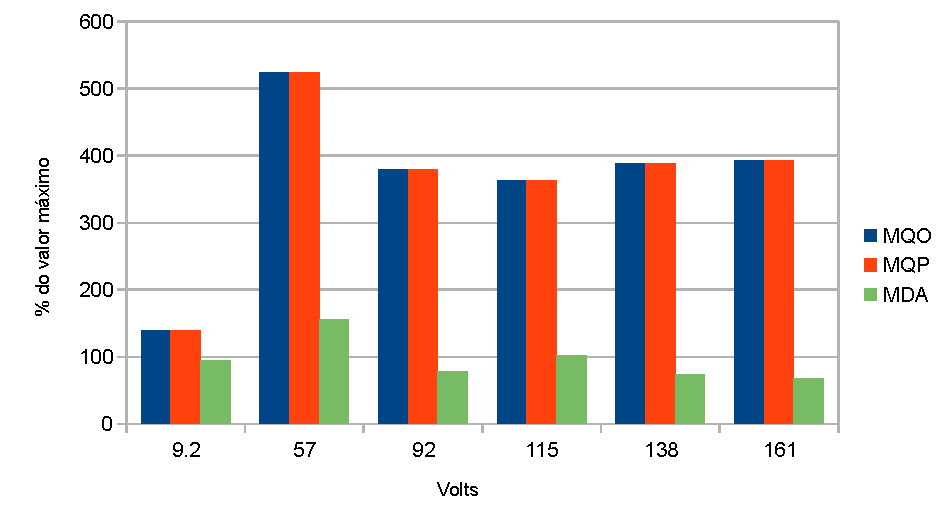
\includegraphics[width=0.9\linewidth]{pictures/max_err_VC_aftercalib60_2nd.pdf}
    \fonte{o autor.}
\end{figure}

Como já é possível perceber, há uma substancial diminuição nos erros, principalmente utilizando a calibração de Mínimos Desvios Absolutos. Apenas os pontos de 57V e 115V os mínimos fornecidos pelo fabricante, o que vale dizer que para os outros quatro pontos o erro manteve-se menor que 0.1$\%$. As médias dos erros após as linearizações em segunda ordem evidenciam ainda mais essa melhora e podem ser observadas na tabela \ref{tab:tabelaerros60Alad2nd}.

\begin{table}[H]
\IBGEtab{%
  \caption[Médias dos erros em relação ao máximo permitido pelo fabricante para o canal de tensão VC em 60 Hz após as calibrações em segunda ordem.]{Médias dos erros em relação ao máximo permitido pelo fabricante para o canal de tensão VC em 60 Hz após as calibrações em segunda ordem.}%
  \label{tab:tabelaerros60Alad2nd}
}{%
  \begin{tabular}{ccc}
  \toprule
  & \textbf{Canal VC} & \\
  \midrule
  \textbf{Erro Médio MQO (\%)} & \textbf{Erro Médio MQP (\%)} & \textbf{Erro Médio MDA (\%)}  \\ 
  \midrule
  359.3539 & 359.3539 &	100.9507 \\
  \bottomrule
\end{tabular}%
}{%
  \fonte{Produzido pelo autor.}%
 % \nota{rd representa o valor lido (em V).}
  %\nota{Esta é uma nota, que diz que os dados são baseados na
 % regressão linear. -- \showfont}%
  %\nota[Anotações]{Uma anotação adicional, que pode ser seguida de várias
  %outras. -- \showfont}%
  }
\end{table}
  
    Procedendo da mesma forma para a calibração em segunda ordem do canal VC com sinais de 50 Hz, são obtidos os resultados expostos na \figref{fig:res_volt2nd50}. Similarmente aos resultados obtidos em 60 Hz, a calibração utilizando o Método de Desvios Absolutos trouxe os melhores resultados observando o erro médio entre todos os pontos, mas ainda assim, este método se mostrou insuficiente para adequar o canal de aquisição com as especificações fornecidas pelo fabricante. A tabela \ref{tab:tabelaerros50Alad2nd} expõe estes resultados.

  \begin{figure}[H]
    \caption{Porcentagem do erro máximo atingido para os sinais de tensão com maior erro por ciclo em 50 Hz após a aplicação do Método dos Mínimos Quadrados Ordinários (MQO), do Método dos Mínimos Quadrados Ponderados (MQP) e do método dos Mínimos Desvios Absolutos (MDA), todos em segunda ordem.}
    \label{fig:res_volt2nd50}
    \centering
    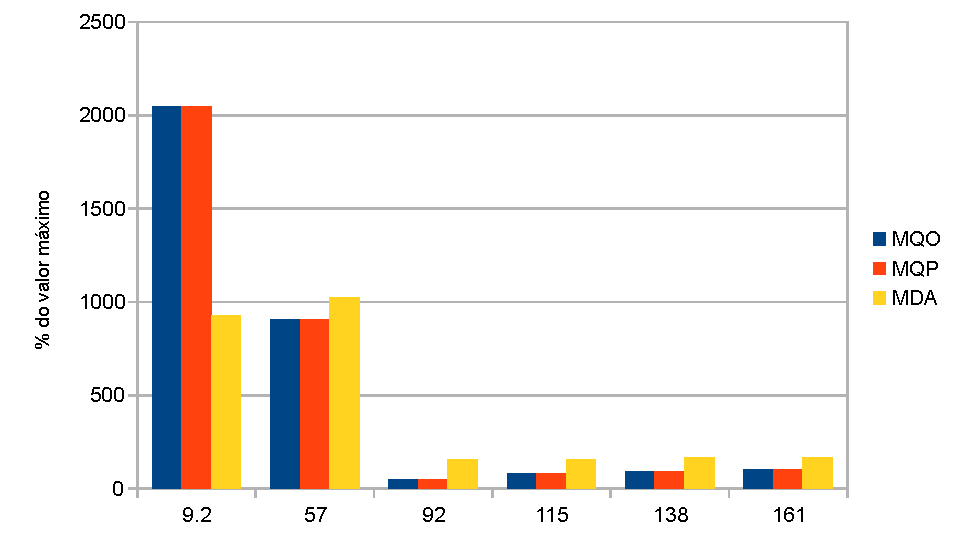
\includegraphics[width=0.9\linewidth]{pictures/max_err_VC_aftercalib50_2nd.pdf}
    \fonte{o autor.}
\end{figure}

\begin{table}[H]
\IBGEtab{%
  \caption[Médias dos erros em relação ao máximo permitido pelo fabricante para o canal de tensão VC em 50 Hz após as calibrações em segunda ordem.]{Médias dos erros em relação ao máximo permitido pelo fabricante para o canal de tensão VC em 50 Hz após as calibrações em segunda ordem.}%
  \label{tab:tabelaerros50Alad2nd}
}{%
  \begin{tabular}{ccc}
  \toprule
   & \textbf{Canal VC}  &\\
  \midrule
  \textbf{Erro Médio MQO (\%)} & \textbf{Erro Médio MQP (\%)} & \textbf{Erro Médio MDA (\%)}  \\ 
  \midrule
  544.9508 & 544.9508 &	433.0842 \\
  \bottomrule
\end{tabular}%
}{%
  \fonte{Produzido pelo autor.}%
 % \nota{rd representa o valor lido (em V).}
  %\nota{Esta é uma nota, que diz que os dados são baseados na
 % regressão linear. -- \showfont}%
  %\nota[Anotações]{Uma anotação adicional, que pode ser seguida de várias
  %outras. -- \showfont}%
  }
  
  
\end{table}

